\documentclass[tikz]{standalone}

\definecolor{n0}{HTML}{785EF0}
\definecolor{End}{HTML}{DC267F}
\definecolor{Corner}{HTML}{FFB000}
\definecolor{NewHex}{HTML}{648FFF}
\definecolor{Reversal}{HTML}{FE6100}

\begin{document}
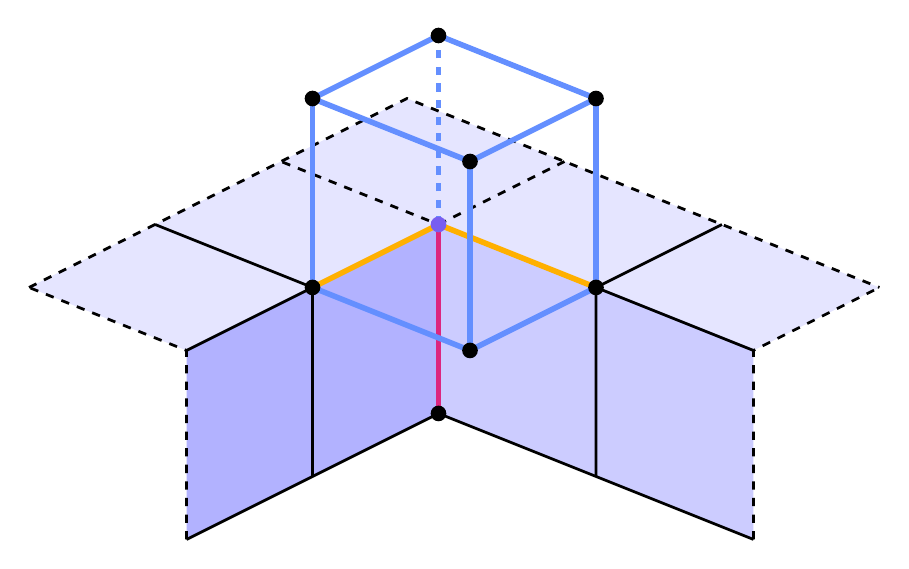
\begin{tikzpicture}[scale=4, x={(0.5cm,-0.2cm)}, y={(0.4cm,0.2cm)}, z={(0.0cm,0.6cm)}]

%%%%%%%%%% Points pour travailler %%%%%%%%%%

 \coordinate (0) at (0,0,0) ;
 \coordinate (1) at (0,1,0) ;
 \coordinate (2) at (0,2,0) ;
 \coordinate (3) at (1,2,0) ;
 \coordinate (4) at (2,2,0) ;

 \coordinate (5) at (0,0,1) ;
 \coordinate (6) at (0,1,1) ;
 \coordinate (7) at (1,1,1) ;
 \coordinate (8) at (0,2,1) ;
 \coordinate (9) at (1,2,1) ;
 \coordinate (10) at (2,2,1) ;
 \coordinate (11) at (-1,0,1) ;
 \coordinate (12) at (-1,1,1) ;
 \coordinate (13) at (-1,2,1) ;
 \coordinate (14) at (-1,3,1) ;
 \coordinate (15) at (0,3,1) ;
 \coordinate (16) at (1,3,1) ;
 \coordinate (17) at (2,3,1) ;

 \coordinate (18) at (0,1,2) ;
 \coordinate (19) at (1,1,2) ;
 \coordinate (20) at (0,2,2) ;
 \coordinate (21) at (1,2,2) ;

  \fill [color=blue!30!white] (0,2,0) -- (0,2,1) -- (0,0,1) -- (0,0,0) -- cycle ;
  \fill [color=blue!10!white] (0,2,1) -- (0,0,1) -- (-1,0,1) -- (-1,3,1) -- (2,3,1) -- (2,2,1) -- cycle ;
  \fill [color=blue!20!white] (0,2,0) -- (0,2,1) -- (2,2,1) -- (2,2,0) -- cycle ;
 
 % Face 1
 \draw [line width=1] (0) -- (2) -- (4) ;
 \draw [line width=1] (5) -- (8) -- (10) ;
 \draw [dashed, line width=1] (11) -- (14) -- (17) ;
 
 \draw [dashed, line width=1] (0) -- (5) -- (11) ;
 \draw [line width=1] (1) -- (6) -- (12) ;
 \draw [dashed, line width=1] (2) -- (8) -- (13) ;
 \draw [dashed, line width=1] (8) -- (15) ;
 \draw [line width=1] (3) -- (9) -- (16) ;
 \draw [dashed, line width=1] (4) -- (10) -- (17) ;

 %%%%%%%%%%% Feature edges %%%%%%%%%%%
 \draw [line width=2, color=End] (8) -- (2) ;
 \draw [line width=2, color=Corner] (8) -- (6) ;
 \draw [line width=2, color=Corner] (8) -- (9) ;

 %%%%%%%%%%% Feature edges %%%%%%%%%%%
 \draw [opacity=0] (8) -- (1) ;
 \draw [opacity=0] (8) -- (3) ;
 
 %%%%%%%%%%% The HEXA created %%%%%%%%%%%
 \draw [line width=2, color=NewHex] (6) -- (7) -- (9) ;
 \draw [line width=2, color=NewHex] (18) -- (19) -- (21) -- (20) -- (18) ;
 \draw [dashed, line width=2, color=NewHex] (8) -- (20) ;
 \draw [line width=2, color=NewHex] (9) -- (21) ;
 \draw [line width=2, color=NewHex] (6) -- (18) ;
 \draw [line width=2, color=NewHex] (7) -- (19) ;

  %%%%%%%%%%% HEXA NODES %%%%%%%%%%%
 \draw (6) node[circle, fill=black, inner sep = 2 pt] {};
 \draw (7) node[circle, fill=black, inner sep = 2 pt] {};
 \draw (8) node[circle, fill=n0, inner sep = 2 pt] {};
 \draw (9) node[circle, fill=black, inner sep = 2 pt] {};
 \draw (18) node[circle, fill=black, inner sep = 2 pt] {};
 \draw (19) node[circle, fill=black, inner sep = 2 pt] {};
 \draw (20) node[circle, fill=black, inner sep = 2 pt] {};
 \draw (21) node[circle, fill=black, inner sep = 2 pt] {};
 \draw (2) node[circle, fill=black, inner sep = 2 pt] {};

\end{tikzpicture}
\end{document}